\chapter{LED load and driver trichologies }
%
%The challenges in powering LED loads are so relevant that have an impact in functionalities and design of the future \emph{Solid-State-Lighting} (SSL) products. So much, that the user adoption of such a beneficial technology by is far slower than comparable disruptive technologies~\cite{11Voger}. In a part, that could be attributed due to the difficulties in achieving the high miniaturization and performance necessary in the LED drivers, at low cost, in order to outcompete the cheaper old technologies.

This chapter starts with an overview of the LED characteristics as a load to give an understanding of the necessary requirements of a LED driver. Subsequently, an overview for the current three driver technologies is given. Linear, switched inductor and switched capacitor, each technology is described, giving the necessary theoretical fundamentals of energy conversion to understand their advantages and limitations.  With the overview for each technology the rational towards \emph{hybrid} converter is given, settling the bases of the converter topology used in this dissertation.

\section{The LED as a load}
\label{sc:LED_load}
A LED is as its acronym stands for a \emph{Light Emitting Diode}. Therefore a LED is a non-linear load with the well-known \emph{voltage-current} ($v-i$) curve of a diode shown in Figure~\ref{fig:led_I-V}. For voltages below the \emph{forward voltage} ($v_{f}$), practically no current flows through it and the LED behaves as an open circuit. For voltages above $v_{f}$ the curve becomes very steep and the current increases dramatically with respect to the voltage, thus the LED behaves similar to a short circuit. The LED has to be supplied at an specific point $P$ in order to provide a desired light output as shown in Figure~\ref{fig:led_I-V}, depending on the bias current light colour and intensity will vary. Due to the steepness in the $v-i$ curve, the practical way to bias a LED is supplying it by a \emph{dc}-current. Owning to the fact that the bast majority of energy sources supply voltage in order two properly supply an LED  it is necessary to select a circuits that converts voltage to current.

\begin{figure}[!h]
\centering
\begin{circuitikz}[american voltages]

    \draw (0,2.5) to[leD*,v=$v$,i=$i$,*-*] (3
    ,2.5) ;

\begin{scope}[xshift=4cm, domain=0:6]
    \draw [->] (0,0) -- (5.5,0) node[anchor=west]{$v$};
    \draw [->] (0,0) -- (0,5.5) node[anchor=east]{$i$};

    %Mark Vth
    \draw (2,2pt) -- (2,-5pt) node[anchor=north] {$v_{f}$};

    %Mark Vthmin and Vt_max
    \def\dvf{0.25}
    \def\dvftop{0.45}

    \draw (1.5,2pt) -- (1.5,-5pt) node[anchor=north] {};
    \draw (2.5,2pt) -- (2.5,-5pt) node[anchor=north] {};
    \draw[dotted] (1.5,0) -- (1.5,\dvftop);
    \draw[dotted] (2.5,0) -- (2.5,\dvftop);
    %Mark Delta Vf
    \draw[pil,>-< ,dotted] (1.25,\dvf) -- (2.75,\dvf);
    \draw (1,\dvf) -- (1.5,\dvf) node[anchor=south east] {$\Delta v_f$};


    %Draw ideal plot
    \draw[thick] (0,0) -- (2,0) -- (4.5,5);

    %Draw lower limit
    \draw[dashed] (0,0) -- (1.5,0) -- (4,5);
    %Draw higher limit
    \draw[dashed] (0,0) -- (2.5,0) -- (5,5);

    %Draw bias point projection
    \draw[dotted] (4,4) -- (4,-0);
    \draw (4,2pt) -- (4,-5pt) node[anchor=north]  {$v_{bias}$};

    \draw[dotted] (4,4) -- (-0,4);
    \draw (2pt,4) -- (-5pt,4) node[anchor=east]  {$i_{bias}$};

    %Draw bias point
    \filldraw (4,4) circle(2pt) node[anchor=south west] {$P$};

    %Draw bias point variations
    \draw (4.5,4)  node[anchor=south west] {};
    \draw (3.5,4)  node[anchor=south west] {};

    %\draw[loosely dotted] (4.5,4) -- (4.5,-0);
    %\draw[loosely dotted] (3.5,4) -- (3.5,-0);
    \draw (4,2pt) -- (4,-5pt) node[anchor=north]  {$v_{bias}$};
    %Mark Vthmin and Vt_max
    \def\bpmi{4.5}
    \def\bpMa{3.5}
    %\draw (1.5,2pt) -- (1.5,-5pt) node[anchor=north] {};
    %\draw (2.5,2pt) -- (2.5,-5pt) node[anchor=north] {};
    %\draw[dotted] (1.5,0) -- (1.5,\dvftop);
    %\draw[dotted] (2.5,0) -- (2.5,\dvftop);
    %Mark Delta Vf
    %\draw[pil,>-< ,dotted] (3.25,\dvf) -- (4.75,\dvf);
    %\draw (4.5,\dvf) -- (5,\dvf) node[anchor=south west] {$\Delta V_{bias}$};

    %Mark Vthmin and Vt_max
    \def\dvf{4}
    %\draw (1.5,2pt) -- (1.5,-5pt) node[anchor=north] {};
    %\draw (2.5,2pt) -- (2.5,-5pt) node[anchor=north] {};
    %\draw[dotted] (1.5,0) -- (1.5,\dvftop);
    %\draw[dotted] (2.5,0) -- (2.5,\dvftop);
    %Mark Delta Vf
    \draw[pil,>-< ,dotted] (3.25,\dvf) -- (4.75,\dvf);
    \draw (4.5,\dvf) -- (5,\dvf) node[anchor=south west] {$\Delta v_{bias}$};


\end{scope}
\end{circuitikz}
\caption{Idealized LED voltage-current characteristic, with the \emph{forward voltage} $v_f$  identified and a projection of the \emph{bias point} P }
\label{fig:led_I-V}
\end{figure}

The characteristics of an LED subjected to variations due to manufacturing tolerances and second order effects at thermal deviations and ageing. Therefore the $i-v$ characteristics is not static and requires the driver to adapt to the load in order to keep the desired light output. The variations in $v-i$ curve can be associated to three main effects. First, $v_f$ has a negative dependence with the temperature, drooping its values as the \emph{pn}-junction temperature increases. Second, the LED has an aging factor which derates the light output over time, and which has to be adjusted by changing the bias point. And third, during production LEDs will vary in colour, flux, and forward voltage; even for products from the same batch. The manufacturers have reduced the tolerances between devices by binning \footnote{Quality control performed at LED production line, where each LED is individual tested and sorted in groups (bins) that have the same electrical and lighting characteristics.}, nevertheless  after binning, the parts are still subjected to some tolerances. For example Table~\ref{tab:vf_values} shows the tolerances in forward voltages for 4 different commercial devices, observing a deviation around $\pm10\%$.

Figure ~\ref{fig:led_I-V} graphically presents how the tolerances in $v_f$ produce a displacement in the $v-i$ characteristic,  which require to modify the $v_{bias}$ within a certain range $\Delta v_{bias}$ in order to keep $i_{bias}$ constant. Despite the variations associated to the load, the driver has at the same time to cope with perturbations and tolerances subjected to the energy supply. The driver has to provide line regulation for static deviations and immunity to high frequency perturbations, without affecting the load. Currently there are three different driver families used to implement LED drivers that are presented in the s subsequent sections.

\begin{table}[!h]
\centering
\caption{Electrical characteristics of different commercial LEDs}
\label{tab:vf_values}
\renewcommand{\arraystretch}{1.5}% Wider
\begin{tabular}{l | c | c |c | c | c | c | c  }
 \multirow{2}{*}{ Model} & \multirow{2}{*}{ Mnf.} & \multicolumn{3}{c|}{ $v_f~[V]$ }  & $i_f$ & Lum. & \multirow{2}{*}{ CCT }  \\ \cline{3-7}
  & & $min.$ & $typ.$ & $max.$ & $[mA]$ & $[lm]$ &  \\
  \midrule
  L130 & Lumileds & 5.8 & 6.1 & 6.6 & 120 & 92 & 4000K\\
  CLA1A & XB-D    &  -  & 2.9 & 3.5 & 350  &  122 & 5000K\\
  NF2L757GR & Nichia & - & 6.32 & 7.1 & 150 & 124 & 3000K\\
  ASMT – M & Avago  & 2.8 & 3.2  & 3.5 & 120 & 350 &  4000K

\end{tabular}
\end{table}

\section{Linear Regulators}
Linear drivers place a shunt element between the source and the load(\emph{i.e} the LED). The shunt element limits the LED current providing the necessary voltage droop between the source and the load. The excess of voltage between the source and the load is dissipated in the series element, literally burned in form of heat; therefore these drivers become very inefficient if the LED voltage is not close to the source. Other limitation is that linear drivers only provide step-down conversion, thus they cannot work when the voltage at the load is higher than the input supply.

\begin{figure}[!h]
\centering
\ctikzset { bipoles/length=1cm}
\begin{subfigure}[t]{.45\textwidth}
    \centering
    \begin{circuitikz} [american voltages,scale=0.65]
    \draw
        (0,0) to[V = $v_{src}$]
        (0,3) to[generic=$r_{series}$,i=$i_o$]
        (5,3) to[R,v=$v_{o}$]
        (5,0) -- (0,0);
    \end{circuitikz}
    \caption{}
    \label{fig:linear_ckt}
\end{subfigure}
\hfill
\begin{subfigure}[t]{.45\textwidth}
    \begin{circuitikz} [scale=0.65]
    \begin{scope}%[xshift = 8cm, yshift=0cm]
        \draw[->] (0,0) -- (4,0) node[anchor=south west] {$  v_o/v_{src} $};
        \draw[->] (0,0) -- (0,3.2) node[anchor=east] {$\eta $};

        %Ticks X
        \draw (3,-5pt) -- (3,2pt)  node[anchor=south west] {$1$};
        \draw (1.5,-5pt) -- (1.5,2pt)   node[anchor=south west] {$0.7$};

        %Ticks Y
        \draw (2pt,2.5) -- (-5pt,2.5) node[anchor=east] {$100\%$};
        \draw (2pt,1.5) -- (-5pt,1.5) node[anchor=east] {$70\%$};

        %Markers
        \draw[dotted] (3,2.5) -- (3,0);
        \draw[dotted] (3,2.5) -- (0,2.5);
        \draw[dotted] (1.5,1.5) -- (1.5,0);
        \draw[dotted] (1.5,1.5) -- (0,1.5);


        \draw[thick] (3,2.5) -- (0,0.5);
    \end{scope}
    \end{circuitikz}
    \caption{}
\label{fig:linear_chr}
\end{subfigure}
\caption{Linear driver, \emph{left}- schematic; \emph{righ}- conversion ratio vs. efficiency characteristics}
\label{fig:linear_drv}
\end{figure}

The circuit of the Figure~\ref{fig:linear_ckt} shows the schematic of a linear driver. The shunt element can be implemented with just a resistor of with an active device. The first will impose a current depending on the input source and the load conditions; the second will provide regulation of the bias point for variations in the source and in the load. Linear drivers are very simple to implement with few components as shown in the schematic of Figure~\ref{fig:ldo_circuit}. They have a very low costs and take almost no area, being indeed the perfect solution for integration.

\begin{SCfigure}[][!h]
    \centering
    \ctikzset { bipoles/length=1cm}
    \ctikzset{tripoles/mos style/arrows}
    \begin{circuitikz} [american voltages,scale=0.65]
    \draw
        (0,0) to[V = $v_{src}$] (0,5)
        (5,5) to[short,i<=$i_o$] (4,5) to[Tnigfete,n=m1] (0,5)
        (5,5) to[leD*]
        (5,2.5) to[R,l=$r_{sense}$]
        (5,0) -- (0,0);
    \draw (3,2.5) node[op amp,xscale=0.5,yscale=-0.5,rotate=-90,](opamp){}
          (opamp.out) -|  (m1.G)
          (opamp.-) |- (4,1.5) |- (5,2.5)
          (opamp.+) |- (2,1.25) node[anchor=east] {$v_{ref}$};
    \draw (7,2.5) node[]{$i_o = \frac{v_{ref}}{r_{sence}}$};

    \end{circuitikz}
    \caption{Low-dropout (LDO) LED driver regulator. The load current $i_o$ is fixed by the voltage $v_{ref}$, despite perturbations in $v_{src}$ and the diode voltage.}
    \label{fig:ldo_circuit}
\end{SCfigure}

The plotted graph in Figure~\ref{fig:linear_chr} presents the variation of the driver efficiency with respect to the conversion ration $m$.
   \begin{equation}
        m = \frac{v_o}{v_{src}}.
   \end{equation}
The efficiency of the driver is the ratio between the input and output power, thus
   \begin{equation}
        \eta = \frac{P_o}{P_i} = \frac{v_o i_o}{v_{src} i_o} = \frac{v_o}{v_{src}} = m,
        \label{eq:linear_reg}
   \end{equation}
which is indeed equal to the conversion ratio. Therefore in a linear regulator the efficiency is subjected to the conversion ratio of the converter, the higher the difference between input and output the lower the efficiency. For instance assuming a minimum efficiency of $80\%$, the maximum accepted conversion ratio is 0.8.


\section{Inductor Based Converters}

\emph{Inductor Based Converters} (IBCs) are switched mode power supplies (SMPS) \footnote{Electronic power supply that provides efficient electric power conversion by commuting between different circuit configurations (modes).}  that employ magnetic passive elements, i.e. inductors and transformers, to store energy and provide efficient electrical power conversion. Therefore the magnetic component is the main passive element in the converter, allowing to process electrical energy by storing in in form of a magnetic field.

IBCs provide step-up and step-down conversion for large dynamic ranges while keeping the efficiency very high. On top of their power conversion capabilities, they can also provide galvanic isolation, which in some mains supplied applications is compulsory in order to guarantee the safety of the users against electrical hazards. These characteristics place these drivers as the preferred solution for the LED industry now a days. Figure~\ref{fig:induct_ckt} shows a \emph{Buck} converter, being it one of the most popular implementations for LED drivers in \emph{dc-dc} applications.  Figure~\ref{fig:induc_chr} presents the regulation characteristic of a generic  inductor based converter. As shown, the theoretical efficiency of these converters is 100\% for all the conversion ratio range. In practice, the parasitics in the components make the efficiency to drop with fluctuations with respect to the point of operation of the converter.

\begin{figure}[!h]
\centering
\ctikzset { bipoles/length=1cm}
\begin{subfigure}[t]{.45\textwidth}
    %\centering
    \raggedright
    \begin{circuitikz} [american voltages,scale=0.65]
    \draw
        (6.5,0) to[short]
        (0,0) to[V = $v_{src}$]
        (0,3) to[gswitch]
        (3,3) to[inductor=${L}$,i=$i_o$]
        (6.5,3);

    \draw (2.5,3) to[gswitch] (2.5,0);

    \draw (6.5,3) to[R,v=$v_{o}$] (6.5,0);

    \end{circuitikz}
    \caption{}
    \label{fig:induct_ckt}
\end{subfigure}
\hfill
\begin{subfigure}[t]{.45\textwidth}
    %\centering
    \begin{circuitikz} [scale=0.65]
    \begin{scope}%[xshift = 8cm, yshift=0cm]
        \draw[->] (0,0) -- (4,0) node[anchor=south west] {$ v_o/v_{src} $};
        \draw[->] (0,0) -- (0,3.2) node[anchor=east] {$\eta $};


        %Ticks Y
        \draw (2pt,2.5) -- (-5pt,2.5) node[anchor=east] {$100\%$};
        \draw (2pt,1.5) -- (-5pt,1.5) node[anchor=east] {$90\%$};

        %Markers
        \draw[dotted] (3,2.5) -- (0,2.5);
        \draw[dotted] (1.5,1.5) -- (0,1.5);


        \draw[thick] (0.5,2.5) -- (3,2.5) node[anchor=south] {$Theoretical$};
        \draw[thick,dashed] (0.5,1.20) parabola[bend at end] (3,1.7) node[anchor=north] {$Real$};
    \end{scope}
    \end{circuitikz}
    \caption{}
\label{fig:induc_chr}
\end{subfigure}
\caption{Inductor based converter, \emph{left} - buck converter schematic; \emph{right} - conversion ration \emph{vs.} efficiency curve comparing the \emph{theoretical} and a \emph{practical} limit. }
\label{fig:inductive_smps}
\end{figure}

The main disadvantage is the use of magnetic components due to their volume and integrability . In practice, inductors dominate the entire volume of the LED drivers as shown in Figure~\ref{fig:smps_driver}. At the same time the three-dimensional nature of these components limit their integrability, specially in standard processes, current research in the field is providing with solutions for power inductors, however they are far to be mature enough for commercial uses.

\begin{SCfigure}[][!h]
\centering
\begin{tikzpicture}
\node[anchor=south west,inner sep=0] (image) at (0,0) {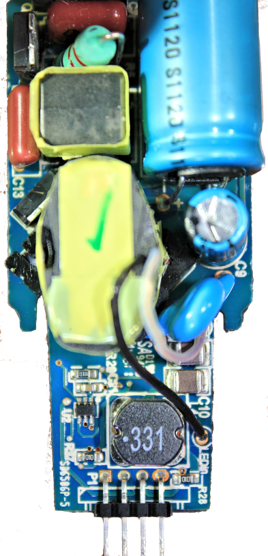
\includegraphics[height=5cm,angle=90]{./0_intro/img/LED_driver.png}};
\begin{scope}[x={(image.south east)},y={(image.north west)}]
%\draw [<-,thick] (0.75,0.5) -- (0.855,0.7)  node [anchor=south west] {Power Magnet};
\draw[black,ultra thick,rounded corners] (0.70,0.3805) rectangle (0.855,0.7);
\draw[black,ultra thick,rounded corners] (0.11,0.1) rectangle (0.28,0.50);
\draw[black,ultra thick,rounded corners] (0.28,0.1) rectangle (0.63,0.62);
\end{scope}
\end{tikzpicture}
\caption{Magnetic components marked with a black square in a mains connected LED driver. These components dominate the volume of the converter.}
\label{fig:smps_driver}
\end{SCfigure}

From the standpoint of view of the switches technology, inductive converters bring yet another disadvantage with respect of the integration of the switches.  Generally, the switches in an inductive converter have to fully block the highest operational voltage of the converter, from the input or the output voltage. Depending on the application, the range is from tens to a few hundreds of volts. Using high voltage devices has three main drawbacks: First, the losses in the devices scale quadratically with the voltage  stress. Second, bad switching performances, because high voltage devices are less efficient and slower switching. Third, the standard VLSI technologies do not offer these \emph{high voltage} (HV) devices and the VLSI technologies that offer them are less performance and more expensive than the dedicated discrete technologies.

\subsection{Energy transfer in switched inductor converters}
%\begin{wrapfigure}{o}{0.7\textwidth}
Inductor based converter are ideally lossless, since the transfer of energy between a voltage source  and an inductor is an adiabatic process, which can be demonstrated using the circuit of Figure~\ref{fig:ind_chrg}.

\begin{figure}[!h]
    \centering
    \begin{subfigure}[b]{.33\textwidth}
    \raggedright
    %\ctikzset { bipoles/length=1cm}
    \begin{circuitikz} [american,scale=0.65]
    \draw
        (0,0) to[battery1 = $v_{src}$]
        (0,3) to[cspst=$s_1$] (2,3) to[short,i=$i$]
        (3,3) to[inductor=${l}$,v=$v_l$]
        (3,0) -- (0,0);
    \draw[white]  (2.5,-2pt) node[anchor=north,font=\footnotesize] {$t+t_{on}$};
    \end{circuitikz}
    \label{fig:induct_charge}
    \end{subfigure}
    \begin{subfigure}[b]{.33\textwidth}
    \raggedright
    \begin{circuitikz} [scale=0.65]
    \begin{scope}%[xshift = 8cm, yshift=0cm]
        \draw[->] (0,0) -- (0,1.25) node[anchor=east] {$ s_1 $};
        \draw[->] (0,0) -- (3.5,0) node[anchor=south] {$  t $};

        \draw[->] (0,1.75) -- (0,3) node[anchor=east] {$ i $};
        \draw[->] (0,1.75) -- (3.5,1.75) node[anchor=south] {$  t $};

        %Ticks Y
        \draw (0.5,0pt) -- (0.5,-2pt) node[anchor=north,font=\footnotesize] {$t_o$};
        \draw (2.5,0pt) -- (2.5,-2pt) node[anchor=north,font=\footnotesize] {$t_o+t_{x}$};

        %Markers
        \draw[dotted] (.5,0) -- (0.5,1.75);
        \draw[dotted] (2.5,0) -- (2.5,2);

        \draw[semithick] (0.5,0) |- (3.25,0.65) ;
        %\draw (1.5,.32) node[font=\footnotesize] {$t_{on}$};
        \fill[gray!50] (0.5,1.75) -- (2.5,2.75)  -- (2.5,1.75);
        \draw[semithick] (0.5,1.75) -- (2.5,2.75) -- (3,3);

        \draw[->] (2,2) to[bend left=45] (1,2.5) node[font=\footnotesize,anchor=south]{$Q_{src}$};

        %\draw[thick,dashed] (0.5,1.20) parabola[bend at end] (3,1.7) node[anchor=north] {$Real$};
    \end{scope}
    \end{circuitikz}

    \end{subfigure}
    \caption{Energy transfer in an inductor.}
    \label{fig:ind_chrg}
\end{figure}
On the one hand, the energy stored in an inductor is given by
\begin{equation}
E_l = \frac{1}{2} l i^2.
\label{eq:e_induct}
\end{equation}
The current flowing in the inductor after switch $s_1$ is closed is given by
\begin{equation}
i(t)= \frac{1}{l} \int v_l dt = \frac{v_{src}}{l}t.
\label{eq:i_inductor}
\end{equation}
Substituting~\eqref{eq:i_inductor} into~\eqref{eq:e_induct}, we can obtain the energy stored in the inductor after closing $s_1$ during the time $t_x$, which results in
\begin{equation}
E_{l,t_x}= \frac{v_{src}^2{t_x}^2}{2l} .
\label{eq:e_l_tx}
\end{equation}
On the other hand, the energy delivered by the energy source $v_{src}$ is given
\begin{equation}
E_{src} = v_{src} q_{src}.
\label{eq:e_src}
\end{equation}
The charge $q_{src}$ delivered by the energy source after closing $s_1$ during a time $t_x$ can be obtained by integrating the inductor current~\eqref{eq:i_inductor},  between $t_o$ and $t_o+t_x$ as
\begin{equation}
q_{src} = \int_t^{t_o+t_x} i(t) dt = \frac{v_{src}}{2l}{t_x}^2 .
\label{eq:q_src}
\end{equation}
|Therefore substituting~\eqref{eq:q_src} into~\eqref{eq:e_src} gives the energy deliver by the source, which gives
\begin{equation}
E_{src,t_x} = \frac{v_{src}^2{t_x}^2}{2l}.
\label{eq:e_src_tx}
\end{equation}
The energy lost while transferring energy between the source and the inductor, is the difference between the energy deliver from the source~\eqref{eq:e_src_tx} and the energy stored in the inductor~\eqref{eq:e_l_tx}, which results in
\begin{equation}
E_{loss} = E_{src,t_x} - E_{l,t_x} = \frac{v_{src}^2{t_x}^2}{2l} - \frac{v_{src}^2{t_x}^2}{2l} =0.
\label{eq:e_loss_l}
\end{equation}
In conclusion, transferring energy between a voltage source and inductor is lossless, and that is why generally inductor based converters achieve very high conversion efficiencies. Nevertheless the parasitics in the components make these converters to do not achieve 100\% efficiencies.

\section{Capacitor Based Converters }
Switched Capacitor Converters (SCCs) are SMPS composed only of switches and capacitors. SCC were initially used for voltage multiplication~\cite{30Cockcroft,44Waidelich,76Dickson} and more recently in applications that need voltage regulation as well~\cite{Ng:EECS-2011-94}. Compared to inductor based converters, the absence of magnetic elements places them in a good position for high density power systems and integrated solutions, such as Power-System-in-Package (PSiP) or Power-System-on-Chip (PSoC).

SCCs have a fixed ratio of conversion between the input and the output determined by the topology. The output voltage of the converter under no load conditions is defined as the \emph{target voltage} ($v_t$). The converter performs at high efficiency when the load is supplied close to the target voltage. Similar to the linear drivers, the efficiency of the converter drops as the difference between the load and target voltage increases. The converter cannot supply a voltage above to the target voltage. Figure~\ref{fig:SCC_ckt} shows a step-down converter with a conversion ratio of one half, thus a 2:1 SCC, and Figure~\ref{fig:SCC_chr} shows the efficiency with respect of the conversion ratio. As the ratio between the input and the output voltages becomes smaller than one-half the efficiency drops linearly, similar like in a linear regulator. For values above one-half the converter is not operative.  A common practice to extend the regulation margins of these converters is to have topologies with a \emph{gear box} that provides multiple ratios of conversion~\cite{2013Ma,2013Breussegem:m_trg}, which are also know as multi-target voltages converters.

% From Figure~\ref{fig:SCC_chr} it can be seen that the efficiency increases as the ration $m$ gets close to the first fixed conversion ration of the converter $m_1$; right after $m_1$ the efficiency drops again dramatically and it again linearly increases as it approaches the second fixed conversion ratio of the converter $m_2$. Beyond $m_2$ the converter does not work.
\begin{figure}[!h]
%\centering
\ctikzset { bipoles/length=1cm}
\begin{subfigure}[t]{.45\textwidth}
    %\centering
    \raggedright
    %\raggedleft
    \begin{circuitikz} [american voltages,scale=0.65]
    \draw
        (6.5,0) to[short]
        (0,0) to[V = $v_{src}$]
        (0,3) to[gswitch]
        (2,3) to[capacitor=${c_1}$]
        (3,3) to[gswitch]
        (5,3) to[short]
        (6.5,3);

    %Parallel switch to ground
    \draw (3.25,3) to[gswitch] (3.25,0);

    %Switch branch to load
    \draw (1.75,3) --
          (1.75,4.5) to[gswitch]
          (5,4.5) --
          (5,3);

    %Load and capacitor C2
    \draw (5,0) to[capacitor=$c_2$,-*] (5,3);
    \draw (6.5,3) to[R,v^=$v_{o}$] (6.5,0);

    \end{circuitikz}
    \caption{}
    \label{fig:SCC_ckt}
\end{subfigure}
\hfill
\begin{subfigure}[t]{.45\textwidth}
    %\centering
    \raggedleft
    %\raggedright
    \begin{circuitikz} [scale=0.65]
    \begin{scope}[xshift = 10cm, yshift=0cm]
            \draw[->] (0,0) -- (4,0) node[anchor=south west] {$  v_o/v_{src} $};
            \draw[->] (0,0) -- (0,3.2) node[anchor=east] {$\eta $};

            %Ticks X
            \draw  (2.5,5pt) -- (2.5,0pt) node[anchor=south west ] {$1/2$};
            %\draw  (3,5pt) -- (3,0pt)   node[anchor=south west ] {$m_2$};
            %\draw (1.5,2pt) -- (1.5,-5pt) node[anchor=north] {$0.7$};

            %Ticks Y
            \draw (2pt,2.5) -- (-5pt,2.5) node[anchor=east] {$100\%$};
            \draw (2pt,1.5) -- (-5pt,1.5) node[anchor=east] {$90\%$};

            %Markers
            \draw[dotted] (2.5,2.4) -- (2.5,0);
            %\draw[dotted] (3,2.3) -- (3,0);
            \draw[dotted] (2.5,2.5) -- (0,2.5);
            %\draw[dotted] (1.5,1.5) -- (1.5,0);
            %\draw[dotted] (1.5,1.5) -- (0,1.5);


            \draw[thick] (0.5,1.4) -- (2.5,2.4); % -- (1.75,1.6) -- (3,2.3)  node[anchor=south] {};
            \draw (10,0)[anchor=north] {};
        \end{scope}
    \end{circuitikz}
    \caption{}
\label{fig:SCC_chr}
\end{subfigure}
\caption{Switched capacitor converter, \emph{left} - 2:1 converter schematic; \emph{right} - conversion ration \emph{vs.} efficiency curve for of a generic multiple  conversion ration stage }
\label{fig:SCC_smps}
\end{figure}

The main limitation of SCCs is that they cannot directly  provide the voltage-to-current regulation, necessary feature of the LED driver. Nevertheless by indirect means the output current can be controlled adding a linear regulator in series with the converter output, compromising the converter efficiency.  Such approach is very popular driver for backlighting LEDs in battery supplied devices, where high  integrability was more relevant than the power efficiency. The backlighint LED driver solution uses a multi-target SCC converter the battery voltage to a voltage above the LED strings, and by means of  linear drivers the output current is adjusted to properly bias the LEDs. Adopting that architecture for general lighting could be a solution, however when scaling the voltages and currents to the requirements of general lighting applications the resulting driver would be infeasible and inefficient.

From the standpoint view of integration the main advantage of these converters is the use no inductors. Integrated capacitors have a better energy density than integrated inductors. The mechanical structure of the capacitors, a stack of metal-isolator-metal, is much easier to replicate on a small scale. With respect to the switches technology, SCCs have the advantage of dividing the operational voltages of  the converter among the different components, thus reducing the voltage stress in the switches and capacitors. Actually, reducing the voltages in the converter has different advantages. First,  capacitors have higher energy density. Second, lower voltage switches have better switching performances and lower associated losses. Finally, lower voltage devices require less silicon area and have a larger offer in the standard very large integration scale (VLSI) processes.



\subsection{Energy transfer in switched capacitor converters}
%\begin{wrapfigure}{o}{0.7\textwidth}
SCCs are by nature lossy, since the transfer of energy between a voltage and a capacitor is a non-adiabatic process, which can be demonstrated using the circuit of Figure~\ref{fig:cap_chrg}.
\begin{figure}[!h]
    \centering
    \begin{subfigure}[b]{.33\textwidth}
    \raggedright
    %\ctikzset { bipoles/length=1cm}
    \begin{circuitikz} [american,scale=0.65]
    \draw
        (0,0) to[battery1 = $v_{src}$]
        (0,3) to[cspst=$s_1$] (2,3) to[short,i=$i$]
        (3,3) to[capacitor=${c}$,v=$v$]
        (3,0) -- (0,0);
    %\draw[white]  (2.5,-2pt) node[anchor=north,font=\footnotesize] {$t_o$};
    \end{circuitikz}
    \label{fig:induct_charge}
    \end{subfigure}
    \begin{subfigure}[b]{.33\textwidth}
    \raggedright
    \begin{circuitikz} [scale=0.65]
    \begin{scope}%[xshift = 8cm, yshift=0cm]
        \draw[->] (0,0) -- (0,1.25) node[anchor=east] {$ s_1 $};
        \draw[->] (0,0) -- (3.5,0) node[anchor=south] {$  t $};

        \draw[->] (0,1.75) -- (0,3) node[anchor=east] {$ v $};
        \draw[->] (0,1.75) -- (3.5,1.75) node[anchor=south] {$  t $};

        %Ticks Y
        \draw (0.5,0pt) -- (0.5,-2pt) node[anchor=north,font=\footnotesize] {$t_o$};
        %\draw (2.5,0pt) -- (2.5,-2pt) node[anchor=north,font=\footnotesize] {$t+t_{x}$};
        \draw (3pt,2.5) -- (-2pt,2.5) node[anchor=east,font=\footnotesize]{$v_{src}$};

        %Markers
        \draw[dotted] (.5,0) -- (0.5,1.75);
        \draw[dotted] (0,2.5) -- (2.5,2.5);

        \draw[semithick] (0.5,0) |- (3.25,0.65) ;
        %\draw (1.5,.32) node[font=\footnotesize] {$t_{on}$};
        %\fill[gray!50] (0.5,1.75) -- (2.5,2.75)  -- (2.5,1.75);
        \draw[semithick] (0.5,1.75) |- (3.25,2.5) ;

        %\draw[->] (2,2) to[bend left=45] (1,2.5) node[font=\footnotesize,anchor=south]{$Q_{src}$};

        %\draw[thick,dashed] (0.5,1.20) parabola[bend at end] (3,1.7) node[anchor=north] {$Real$};
    \end{scope}
    \end{circuitikz}

    \end{subfigure}
    \caption{Energy transfer in a capacitor.}
    \label{fig:cap_chrg}
\end{figure}

On the one hand, the energy stored in a capacitor is given by
\begin{equation}
E_c = \frac{1}{2} c v^2.
\label{eq:e_cap}
\end{equation}
After closing the switch at $t_o$, the capacitor is charged at $v_{src}$.  The charge delivered by the source $q_{src}$ to the capacitor is given by
\begin{equation}
q_{src}= c~v_{src},
\label{eq:q_src_cap}
\end{equation}
hence the energy stored in the charged capacitor results in
\begin{equation}
E_{c^+} = \frac{1}{2} \frac{q_{src}}{v_{src}}  {v_{src}}^2 = \frac{1}{2}q_{src}~v_{src}.
\label{eq:e_cap+}
\end{equation}
On the other hand, the energy delivered by the energy source is just
\begin{equation}
E_{src} = v_{src} q_{src}.
\label{eq:e_src_c}
\end{equation}
The energy lost while transferring energy between the source and the capacitor, is the difference between the energy deliver from the source~\eqref{eq:e_src_c} and the energy stored in the capacitor~\eqref{eq:e_cap+}, which results in
\begin{equation}
E_{loss} = E_{src} - E_{c^+} = v_{src}~q_{src}  - \frac{1}{2}q_{src}~v_{src}  = \frac{1}{2}q_{src}~v_{src}.
\label{eq:e_loss_l}
\end{equation}
In conclusion, transferring energy between a voltage source and a capacitor is a lossy process. Actually, half of the used energy is lost, and the other half is stored in the capacitor. The energy lost is dissipated in the resistive elements of the current path such as the \emph{on}-channel resistance and track resistances.










\section{Overview in integration of LED drivers }
With regard to the integration of power supplies, we can indemnify two clear approaches, Power System on Chip (PSoC), and  Power System in Package (PSiP). PSoCs integrate all converter functions, power train and control, in a single die, using the available in-die reactive components. Currently, the standard VLSI processes offer capacitors and inductors with low energy densities, generally provided for radio frequency (RF) proposes. PSiPs integrate the converter in a single integrated circuit package, allowing to use multiple dies with different technologies and dedicated miniaturized discrete components. Currently there are few commercially available PSiP LED drivers offered by \emph{Linear Technology}.

There is yet another approach in integration of power supplies, where the IC integrates the power train and the control, using off-package  passive components. In reality, this is a widely adopted and dominant solution among the different IC manufacturers that provide LED dedicated drivers for the three main applications: Screen back-lighting, general lighting and automotive. In order to fulfil these applications manufacturers offer two possible IC solutions, stand-alone controllers, and integrated power train and controller. These application specific drivers facilitates the development by reducing component count and design time, however the flexibility in the design of the new topologies that help integrability and improve the power density is very limited since the driver topologies are already fixed by the available ICs.
\begin{figure}[!ht]
\centering
\ctikzset{bipoles/length=1cm}
\tikzstyle{hs_s}=[shift={(-0.125,0)}]
\begin{circuitikz} [american,scale=0.65]
   \draw[thick,dashed] (2.5,0.25) --
                (2.5,6.5) --
                (11.5,6.5) --
                (11.5,0.25) --
                (2.5,0.25);

    %Draw SCC block with capacitors
    \draw (3,1) --
          (3,6) --
          (5,6) --
          (5,1) --
          (3,1);

    \draw (11.5,6.5) node[anchor=north east] {IC PACKAGE};
    \draw (3.5,3.5) node[rotate=90] {SMPS};
    \draw (4.5,3.5) node[rotate=90,font=\footnotesize] {(with off-chip passives)};

    \draw (5,5.5) to[short,-o] (12,5.5)  -- (14,5.5);
    \draw (12.5,5.5) -- (12.5,5.25)  to[C,/tikz/circuitikz/bipoles/length=0.75cm] (12.5,4.75) node[sground,scale=0.75]{};

    \draw (4,1) to[short,-o] (4,0) -- (4,-0.25)  node[sground,scale=0.75]{};

   %Draw linear drivers
   \draw  (4,0.5) -- (11,0.5) ;

   %First transitor
   \draw   (10,0.5) to[R,/tikz/circuitikz/bipoles/length=0.5cm]
           (10,1.5)-- (10,2.5) node[npn,anchor=E,scale=0.5](npn1){}
           (npn1.C) -- (10,3.75) to[short] (12,3.75)
           (8.5,1.5) -- (10,1.5);


   %Second transitor
   \draw  (11,0.5) to[R,/tikz/circuitikz/bipoles/length=0.5cm]
          (11,1.5) -- (11,2) node[npn,anchor=E,scale=0.5](npn2){}
          (npn2.C) -- (11,3.25) to[short] (12,3.25)
          (8.5,1.75) -- ([hs_s]8.5,1.75 -| 10,1.5 ) arc(180:0:0.125) --   (11,1.75);


   %Controller box
   \draw (5.5,1) -- (8.5,1) -- (8.5,4) -- (5.5,4) -- (5.5,1);
   \draw (5.75,2.5) node[anchor=west, text width = 1.75cm,font=\footnotesize]{Intensity Controller};
   \draw (npn2.B) -| (8.5,3);
   \draw (npn1.B) -| (8.5,3);

   %LEDs
   \draw (14,5.5) to[short] (14,5.5)
                    to[leD*,/tikz/circuitikz/bipoles/length=0.75cm] (14,3.75) to[short,-o] (12,3.75);

   \draw (14,5.5) -- (15.5,5.5)
                    to[leD*,/tikz/circuitikz/bipoles/length=0.75cm] (15.5,3.75) -- (15.5,3.25) to[short,-o] (12,3.25);

   %Add battery

   \draw (-1,-0.25)  node[sground,scale=0.75]{} -- (-1,0) to[V = $v_{src}$] (-1,5.5)
         to[short,-o] (2,5.5) -- (3,5.5);

  % \draw (3,5) to[short,-o] (2,5) -- (1.25,5) to[C,l_=$c_2$,/tikz/circuitikz/bipoles/length=0.75cm] (1.25,3.5) to[short,-o] (2,3.5) -- (3,3.5);
%   \draw (3,3) to[short,-o] (2,3) -- (1.25,3) to[C,l_=$c_1$,/tikz/circuitikz/bipoles/length=0.75cm] (1.25,1.5) to[short,-o] (2,1.5) -- (3,1.5);


    \end{circuitikz}
    \caption{Block diagram of a commercial LED driver IC used in back-lighting applications.}
    \label{fig:backlight_LED}
\end{figure}

In back-lighting, the commercial ICs integrate a power train, control unit and a communication interface. Back-lighting applications require multiple LED channels, therefore these drivers implement the power train  architecture shown in Figure~\ref{fig:backlight_LED}. A SMPS (inductive or capacitive) converts the supply voltage to a voltage above the LED strings, and a linear regulator is in series with each LED string channel enabling to control individually the currents for each channel~\cite{2008Yuequan,07Feng}. In general lighting and automotive applications the dedicated commercial ICs implement only inductor based converters such as back, boost, flyback, etc., providing just a solution for the power conversion point of view without integrating other functionalities. With an innovative approach and looking towards the future connected lamps, \emph{Gooee}~\cite{web:Gooee} provides a two chip solution a LED driver chip with off-chip passives, and a dedicated $\mu$Controller unit. The final solution enables a LED lamp with smart functionalities such as sensing, data logging and cloud connectivity.


\section{ Summary}

A background of the different driver technologies and the state-of-the-art of LED driver integration was given in order to contextualize better our research question:

\emph{
\centering 
 Could just a SCC drive a High-Brightness LED?
 }

Based on the aforementioned characteristics, a SCC driver seems to be, a priori, the correct choice, when looking them in terms of regulation and voltage conversion. These converters provide a voltage-to-voltage conversion in discrete steps, and as previously mentioned, a LED load is generally supplied by current due to their abrupt $v-i$ characteristics. On possible solution, would be to design a SCC with enough conversion steps, however the necessary granularity in the conversion steps would make the converter practically infeasible due to the large number of capacitors and switches. Another solution, would be to combine the SCC with a linear regulator, what is indeed currently a commercial solution in screen back-lighting for low-power battery supplied devices, but it the SCC stage is been replaced for an inductive stage in applications using a higher power, and high brightness LEDs. Nevertheless, a SCC based driver would be an interesting candidate in terms of integration, since SCCs allow to address higher-voltages applications using lower-voltages process. What might enable to implement a power converter using standard CMOS low-voltage integration processes
 
In order to overcome limitations of the SCC while keeping a converter with high efficiency and a tight current regulation, an inductive converter seemed to be a more suitable solutions since they excel in both characteristics. However as the voltages addressed by the converter increase, the switches in the converter also scale in voltage, making not possible to implementing converters in a standard CMOS low-voltage process and harming the integrability of the converter. That is why, we found a compromise solution between both SMPS technologies by combining a SCC with an inductor, in what we defined as a \emph{Hybrid-Switched Capacitor Converter} abbreviated in H-SCC. 

The H-SCC implements converter where the power train is a SCC, and the LED is supplied through an inductor connected to one of the internal nodes of the SCC. The proposed solution enables a converter suitable to integration, providing high efficiency and current regulation, and at the same time, reducing the size of the inductor compared to an inductive converter. In conclusion, the H-SCC has been the selected topology for a high-integrated and miniaturized LED driver, and the center of this dissertation.   



\bibliographystyle{plainnat}
\bibliography{references} 